\documentclass[
	preprint,%twocolumn
	aps,
	prb,
	showpacs,	
	amsmath, amssymb]{revtex4-2}
%---packages----------------------------------------------------------
%\usepackage[top=1.25in, bottom=1.25in, left=1.25in, right=1.25in]{geometry}
\usepackage{bm}
\usepackage{graphicx}
\usepackage{hyperref}% add hypertext capabilities
\hypersetup{colorlinks=true, 
			citecolor=blue, 
			urlcolor=blue, 
			linkcolor=blue}
\pdfstringdefDisableCommands{\let\bm=\relax}
\usepackage{scalerel}
\usepackage{cleveref}
\usepackage{tikz} % flow chart
\usetikzlibrary{positioning, shapes.geometric}


%--setups--------------------------------------------------------------
\DeclareRobustCommand{\xjoinrel}{\mathrel{\mkern-4mu}}
\DeclareRobustCommand{\gong}{\hstretch{1.25} {\boldsymbol{\mathrel{|} \xjoinrel\mathrel{-} \xjoinrel\mathrel{|}}}}
%\DeclareRobustCommand{\gong}{\hstretch{1.25} {\boldsymbol{\vdash \xjoinrel\dashv }}}
%\DeclareRobustCommand{\wang}{\hstretch{1.25} {\boldsymbol{\vdash \xjoinrel \mathrel{+} \xjoinrel\dashv }}}
\DeclareRobustCommand{\wang}{\hstretch{1.25} {\boldsymbol{\mathrel{|}  \xjoinrel\mathrel{-} \xjoinrel\mathrel{|} \xjoinrel\mathrel{-} \xjoinrel\mathrel{|}}}}
\DeclareRobustCommand{\+}{\hstretch{1.25} {\boldsymbol {\mathrel{+}}}}
\DeclareRobustCommand{\manyplus}{\hstretch{1.25} {\boldsymbol{ \mathrel{+}\xjoinrel \mathrel{+}\xjoinrel\mathrel{+} \xjoinrel\mathrel{+}}  }}
\DeclareRobustCommand{\l}{\hstretch{1.25} {\boldsymbol {\vdash }}}
\DeclareRobustCommand{\r}{\hstretch{1.25} {\boldsymbol {\dashv }}}
%\DeclareRobustCommand{\tu}{\hstretch{1.25} {\boldsymbol {\mathrel{+} \xjoinrel\dashv }}}
\DeclareRobustCommand{\tu}{\hstretch{1.25} {\boldsymbol{\mathrel{-} \xjoinrel\mathrel{|} \xjoinrel\mathrel{-} \xjoinrel\mathrel{|}}}}
%\DeclareRobustCommand{\tl}{\hstretch{1.25} {\boldsymbol {\xjoinrel\dashv \mathrel{+}}}}
\DeclareRobustCommand{\tl}{\hstretch{1.25} {\boldsymbol{\mathrel{|}  \xjoinrel\mathrel{-} \xjoinrel\mathrel{|} \xjoinrel\mathrel{-} }}}

\newcommand{\tr}{ {\rm Tr} }
\newcommand{\I}{ {\mathbb I} }
\newcommand{\im}{ {\mathrm{Im}} }
\newcommand{\re}{ {\mathrm{Re}} }
\newcommand{\sgn}{ {\mathrm{Sgn}} }
\newcommand{\Y}{ {\mathcal{Y}} }
\newcommand{\C}{ {\mathcal{C}} }
\newcommand{\Cbar}{ {\bar{\mathcal{C}}} }
\newcommand{\D}{ {\mathcal{D}} }
\newcommand{\Dbar}{ {\bar{\mathcal{D}}} }
\newcommand{\B}{ {\mathcal{B}} }
\newcommand{\N}{ {\mathcal{N}} }

%=======================================================================
%=======================================================================
\begin{document}
\title{Notes: Nevanlinna analytical Continuation Method}
\author{Shuang Liang}
\email{sliang@iphy.ac.cn}
\affiliation{Institute of Physics, Chinese Academy of Sciences}


%\author{Shuang Liang}
%\affiliation{Institute of Physics, Chinese Academy of Sciences}
%\email{sliang@iphy.ac.cn}

\date{\today}
\begin{abstract}
	This is the abstract.
\end{abstract}


\maketitle
\tableofcontents

\newpage
%=====================================================================
%=====================================================================
\section{The analytic continuation problem}
\label{sec:the-analytic-continuation-problem}

The analytic continuation problem seeks   
to extract real frequency dynamical information from
imaginary-time correlation functions $G(\tau)$ data.
Technically, this is a highly nontirvial task\cite{jarrell1996bayesian}. To 
see this, we use the relation between $G(\tau)$ and $A(\omega)$
\cite{jarrell1996bayesian,XiaoLRT}:
\begin{equation}\label{eq:gt-Aw}
	G(\tau) = \int_{-\infty}^{\infty} d\omega
		\frac{e^{-\tau \omega }}{1 - \lambda e^{-\beta \omega}}
		A(\omega)
		= \int_{-\infty}^{\infty} d\omega
		K(\tau, \omega) A(\omega)
\end{equation}
where $K(\tau, \omega) = \frac{e^{-\tau \omega }}{1 - \lambda e^{-\beta \omega}}$
is the kernel, $\lambda =\pm 1$ for bosons/fermions respectively. One may consider to solve the problem by firstly 
discretize $\tau$ and $\omega$ and get:
\begin{equation}
	G(\tau_i) = \sum_{j=1}^{N_\omega} K_{ij} A(\omega_j)
\end{equation}
Then do SVD decomposition of rectangular matrix $K$, write
$K_ij = U_{il} \lambda_l V_{lj}$. Finally the spectral function 
reads
\begin{equation}
	A(\omega_j) = \sum_{l=1}^{N_\tau} \frac{1}{\lambda_l} V_{ij}
		\sum_{i=1}^{N_\omega} G(\tau_i) U_{il}
\end{equation}
It seems fine at the first glanse. However, if we consider 
the properties of $K(\tau, \omega)$, we would notice that it 
is highly sigular since it is exponentially small for large 
$|\omega|$, so small errors $G(\tau)$ would be amplified by
exponentially small $\lambda_l$. This problem is well-known
ill-posed\cite{acton1997numerical, peschel1999density} and 
enormous efforts have been made\cite{}.


%=====================================================================
%=====================================================================
\section{How to solve?}
\label{sec:how-to-solve}

$\cdots$

Here we introduce the recently developed Nevanlinna 
analytic continuation method\cite{fei2021nevanlinna}.      
%=====================================================================
%=====================================================================
\section{Nevanlinna analytic continuation method}
\label{sec:nevanlinna-analytical-continuation-method}

The Nevanlinna analytic continuation method\cite{fei2021nevanlinna} 
is an interpolation method. The key step is to build the conformal mappings 
from the open upper half of the complex plane $\C^+$ 
to a closed unit disk $\Dbar$ in the complex plane and 
make use of the Schur algorithm
\cite{schur1917potenzreihen,schur1918potenzreihen,dym2003contributions} 
to do the interpolate.

%=====================================================================
\subsection{Schur Algorithm}
\label{subsec:schur-algorithm}

Schur Algorithm was introduced by I. Schur\footnote{Schur 
	published under the name of both I. Schur, 
	and J. Schur, the latter especially in  
	\textit{Journal für die reine 
	und angewandte Mathematik}. This has led to some confusion.
	See:\href{https://en.wikipedia.org/wiki/Issai_Schur#cite_note-2}{Issai Schur}} 
in Section 1 of Ref.\cite{schur1917potenzreihen}.
Here we list the main results we need while
for a detailed introduction, see Ref.\cite{dym2003contributions}. 

A Schur class($\mathcal{S}$) consists of the Schur functions, which are the 
\href{https://en.wikipedia.org/wiki/Holomorphic_function}{holomorphic functions} 
from the open unit disk $\D$ to 
the closed unit disk $\Dbar$. 
For a given Schur function $s_0(z)$, the Schur algorithm defines a set of
$\{s_j(z) \in \mathcal{S}\}_{0\leq j <\infty}$ starting from $s_0(z)$ by the recurrence relation:
\begin{equation}\label{eq:schur-function-recursion}
	zs_{j+1}(z) = \frac{s_j(z) - \gamma_j}{1 - \gamma_j^* s_j(z)}
\end{equation}
where $s_j \in \mathcal{S}$ and $\gamma_j \equiv s_j(0)$ are called Schur 
parameters and $|\gamma_j| \leq 1$. 

On the other hand, given an arbitrary strictly contractive sequence 
of Schur parameters $\{\gamma_0, \gamma_1, \dots, \gamma_j, \dots\} \in \D$, 
one can construct a unique Schur function $s_0(z)$ by means of a continued 
fraction algorithm. In which we use the inverse relation of
\cref{eq:schur-function-recursion}
\begin{equation}\label{eq:inv-schur-function-recursion}
	s_j(z) = \frac{\gamma_j + zs_{j+1(z)}}{1 + \gamma_j^* z s_j(z)}
\end{equation}
to construct the $n$-th Schur approximant, 
which we will denote by 
$s_0(z; \gamma_0,\gamma_1, \dots, \gamma_n)$. Namely, we write:
\begin{align}\label{eq:schur-continued-fraction}
\begin{split}
	&s_n(z;\gamma_n) = \gamma_n \\
	&s_j(z;\gamma_j,\gamma_{j+1},\dots \gamma_n) 
	= \frac{\gamma_j + zs_{j+1}(z;\gamma_{j+1},\dots \gamma_n)}
		{1 + \gamma_j^* z s_{j+1}(z;\gamma_{k+1},\dots \gamma_n)}
\end{split}
\end{align}
where $j = n-1, n-2, \dots, 1, 0$.

The Schur algorithm can used to solve the interpolation problem in $\D$. 
For given $\{\Y_0, \Y_1, \dots ,\Y_N\} \in \D$ 
and $\{\gamma_0, \gamma_1, \dots ,\gamma_N\} \in \D$, the Schur function 
 $s:\D \to \D$ and $s(\Y_j) = \gamma_j$ 
for $j = 0,1,\dots,N$ can be easily constructed by combining 
\cref{eq:schur-continued-fraction} and the linear fractional transform 
$f(z, \Y_j) = \frac{z - \Y_j}{1 - z\Y_j^*}$:
\begin{align}\label{eq:schur-interpolation}
	\begin{split}
		&s_N(z;\gamma_N) = \gamma_N \\
		&s_j(z;\gamma_j,\gamma_{j+1},\dots \gamma_N) 
		= \frac{\gamma_j + f(z,\Y_{j})s_{j+1}(z;\gamma_{j+1},\dots \gamma_N)}
			{1 + \gamma_j^* f(z,\Y_{j})s_{j+1}(z;\gamma_{k+1},\dots \gamma_N)}
	\end{split}
\end{align}
where $j = N-1, N-2, \dots, 1, 0$.


%=====================================================================
\subsection{Generalized Schur Algorithm}
\label{subsec:generalized-schur-algorithm}





%=====================================================================
\subsection{The Nevanlinna–Pick theorem}
\label{subsec:pick-theorem}

Wikipedia: 
\href{https://en.wikipedia.org/wiki/Nevanlinna%E2%80%93Pick_interpolation}{The Nevanlinna–Pick theorem}

The Nevanlinna–Pick theorem states the following.
Given the initial data consisting of $n$ points 
$\{\lambda_0, \dots, \lambda_{n-1} \} \in \D$ and target data
$\{z_0, \dots, z_{n-1} \} \in \D$, there exists 
a holomorphic function $g(z): \D \to \Dbar$ 
such that $g(\lambda_j) = z_j$ for all $j$, if and only if 
the Pick matrix
\begin{equation}
	P_{jk} = \frac{1-z_k^* z_j}{1 - \lambda_j^* \lambda_k}
\end{equation}
is positive semi-definite. Furthermore, the function $g(z)$ is 
unique if and only if the Pick matrix has zero determinant.


%=====================================================================
\subsection{Interpolation of Green's functions}
\label{subsec:interpolation-of-GF}

The retared Green's function $G^R(\omega + i\eta)$ and the Masubara 
Green's function $G(i\omega_n)$ can be expressed consistently by replacing 
the variables $i\omega_n$ and $\omega + i\eta$ with a single complex 
variable $z$. $G(z)$ is analytic in the upper half plane. 
Our problem is that once we have Masubara frequencies $\{i\omega_n\} \in \C^+$ 
and target data $\{ G(i\omega_n)\} \in \C$, where $\C$ is 
the complex plane, how can we get interpolate them and get the 
holomorphic function $G(z)$?

Based on the knowledge of Schur function, if we can find maps 
to map the initial data set $\{ G(i\omega_n)\}$
from $\C^+$ to $\D^+$ and the target 
target data $\{ G(i\omega_n)\}$ from $\C$ to $\bar{\D^+}$, 
then we can apply the Schur function. 
To accomplish this task, we can to make use of the generalized 
Schur algorthm\cite{adamyan2003reconstruction}. It generalize the 
method from $g(z) \in \mathcal{S}$ to all contractive functions 
$\theta(z) \in \B$, which 
are holomorphic functions mapping from $\mathcal{C^+}$ 
to $\Dbar$.	









%=====================================================================
\section{old}



In this method, one should firstly using 
conformal transforms to map the Masubara Green's functions $\mathcal{G}$, 
which is analytic in the upper half of the complex plane $\C^+$ and 
contains singularities in the lower half plane, to a closed unit disk 
$\Dbar$ in the complex plane. The mappings are shown in \cref{fig:conformal-map}. 
It becomes a Schur class($\mathcal{S}$) 
function and would have a continued fraction expansion where the parameters 
can be rescrsively defined\cite{schur1918potenzreihen}. Then one can 
apply the Nevanlinna iterative algorithm to interpolate the Schur 
functions\cite{nevanlinna1919uber}.
Finally, one can do a inverse conformal transform back to $\C^+$ and 
obtains $\mathcal{G}(z)$, it's then natural to do analytic continuation 
$z \to \omega + i0^+$. The calculation process is shown in \cref{fig:calculation-flow-chart}.

\begin{figure}[htbp]
	\centering
	\begin{minipage}[t]{0.7\linewidth}
		\centering
		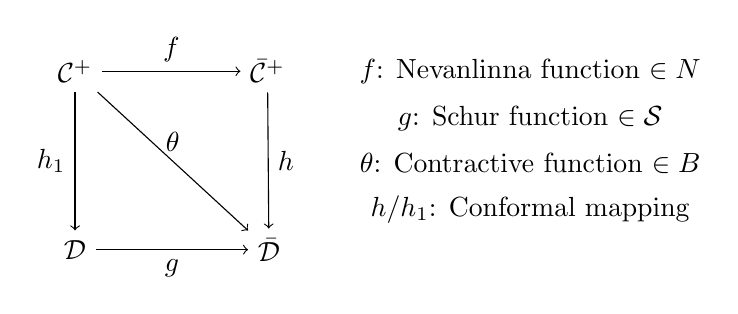
\begin{tikzpicture}[node distance=50pt]
			\node[draw=none,fill=none]  (C)  {$\C^+$};
			\node[draw=none,fill=none, right=of C]  (Cbar)  {$\Cbar^+$};                 
			\node[draw=none,fill=none, below=of C]  (D)     {$\D$};               
			\node[draw=none,fill=none,right=55pt of D]  (Dbar)  {$\Dbar$};
		
			\draw[->] (C)  -- node[above] {$f$} (Cbar) ;
			\draw[->] (C)  -- node[left] {$h_1$} (D) ;
			\draw[->] (C)  -- node[above] {$\theta$} (Dbar) ;
			\draw[->] (Cbar) -- node[right] {$h$} (Dbar) ;
			\draw[->] (D) -- node[below] {$g$} (Dbar) ;

			\node[draw=none,fill=none, right=20pt of Cbar] (f) {$f$: Nevanlinna function $\in N$};
			\node[draw=none,fill=none, below=1pt of f]  (g)  {$g$: Schur function $\in \mathcal{S}$};                 
			\node[draw=none,fill=none, below=1pt of g]  (t)     {$\theta$: Contractive function $\in B$};               
			\node[draw=none,fill=none,below=1pt of t]  (h)  {$h/h_1$: Conformal mapping};
		\end{tikzpicture}
	\end{minipage}
	\caption{Conformal mappings}
	\label{fig:conformal-map}
\end{figure}

\begin{figure}[htbp]
	\centering
	\begin{minipage}[t]{0.9\linewidth}
		\centering
		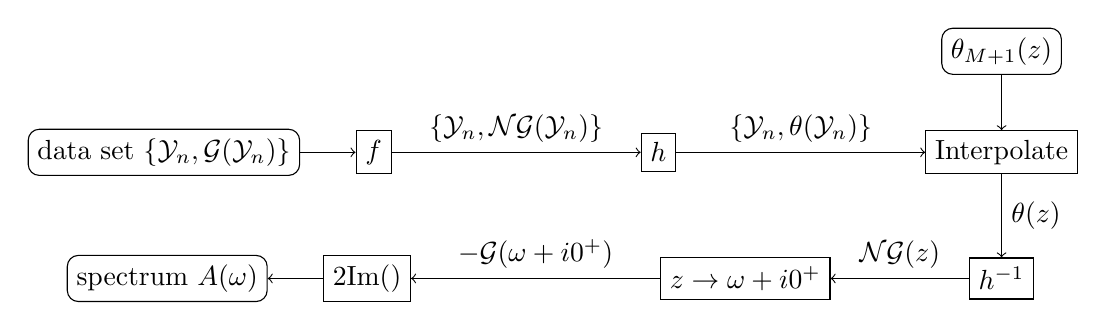
\begin{tikzpicture}[node distance=90pt]
			\node[draw,rounded corners]  (start)  {data set $\{\Y_n, \mathcal{G}(\Y_n)\}$};
			\node[draw,right=20pt of start]  (f)  {$f$};                 
			\node[draw, right=of f]  (h)     {$h$};               
			\node[draw,right=of h]  (interpolate)  {Interpolate};
			\node[draw,rounded corners,above=20pt of interpolate]  (tm)  {$\theta_{M+1}(z)$};
			\node[draw, below=30pt of interpolate]  (invh)  {$h^{-1}$};
			\node[draw, left=50pt of invh]  (ac)  {$z \to \omega + i0^+$};
			\node[draw, left=of ac]  (imag)  {$2\im()$};
			\node[draw, rounded corners, left=20pt of imag]  (end)  {spectrum $A(\omega)$};

			\draw[->] (start) -- (f) ;
			\draw[->] (f)  -- node[above] {$\{\Y_n, \mathcal{NG}(\Y_n)\}$} (h) ;
			\draw[->] (h)  -- node[above] {$\{\Y_n, \theta(\Y_n)\}$} (interpolate) ;
			\draw[->] (tm) -- (interpolate) ;
			\draw[->] (interpolate) -- node[right] {$\theta(z)$} (invh) ;
			\draw[->] (invh) -- node[above] {$\mathcal{NG}(z)$} (ac) ;
			\draw[->] (ac) -- node[above] {$-\mathcal{G}(\omega + i0^+)$} (imag) ;
			\draw[->] (imag) -- (end) ;
		\end{tikzpicture}
	\end{minipage}
	\caption{Calculation flow chart}
	\label{fig:calculation-flow-chart}
\end{figure}

For fermionic Green's functions, the mapping from $\C^+$ to 
$\bar{\C^+}$ is simple. Since $\im \mathcal{G}(z) \leq 0$ if 
$z \in \C^+$, the mapping is just to take 
$\mathcal{G} \to -\mathcal{G} = \mathcal{NG}$ and $\mathcal{NG} \subset N$. While for 
bosonic Green's functions, this mapping is a little bit complicated and 
we will discuss in the next section. The data set we have is 
$\{i\omega_n, \mathcal{G}(i\omega_n)\}$, here we denote $\Y_n = i\omega_n$ 
and $\C_n = \mathcal{NG}(i\omega_n) = -\mathcal{G}(i\omega_n)$. 

Then we use the Möbius transform
\begin{equation}\label{eq:Mobius-transform}
	h(z) = \frac{z - i}{z + i}
\end{equation}
to map $\C_n \subset N$ to 
$\theta(\Y_n) = h(\C_n) \subset \Dbar$. 
The recursive final $\theta(z)$ can conveniently be written in a
matrix form:
\begin{equation}\label{eq:recursive-theta}
	\theta(z)[z;\theta_{M+1}(z)] 
		= \frac{a(z)\theta_{M+1}(z) + b(z)}{c(z)\theta_{M+1}(z) + d(z)}
\end{equation}
where
\begin{equation}\label{eq:factor-matrix}
	\left(
		\begin{matrix}
			a(z) & b(z) \\
			c(z) & d(z)
		\end{matrix}
	\right) = \prod_{n=1}^M
	\left(
		\begin{matrix}
			h_1(z, \Y_j) & \phi_j \\
			\phi_j^* h_1(z, \Y_j) & 1
		\end{matrix}
	\right)
\end{equation}
where $h_1(z, \Y_n) = \frac{z - \Y_n}{z -\Y_n^*}$ 
is a conformal map form $\C^+$ to $\D$. $\theta_j(z)$ is 
the interpolation function of $j$-th step and
$\phi_j = \theta_j(\Y_j)$. There is a freedom to choose $\theta_{M+1}(z)$.
One can use this freedom to select the “best” of all consistent spectral functions.

%=====================================================================



\appendix
%=====================================================================
%=====================================================================
\section{Conformal transforms}
\label{app:conformal-transforms}

\subsection{The linear fractional transform}
\label{appsub:linear-fractional-transform}
The linear fractional transform is:
\begin{equation}\label{eq:linear-fractional-transform}
	f(z, \Y) = \frac{z - \Y}{1 - z\Y^*}
\end{equation}

It is a one to one mapping of the open unit disk $\D$ onto 
itself and a one to one mapping of the unit circle $\mathcal{T}$.
It maps point $\Y$ to the center of $\D$.


\subsection{The Mobius transform}
\label{appsub:mobius-transform}
The mapping from $\C^+/\bar{\C^+}$ to 
$\D^+/\bar{\D^+}$ is called Mobius transform.
It has the form:
\begin{equation}\label{eq:def-mobius-transform}
	h(z, \Y)  = \frac{z - \Y}{z - \Y^*}
\end{equation}
where $\Y \in \Cbar^+$ and $\Y \neq 0$. We can easily prove that 
$|h(z, \Y)| \leq 1$ for $z \in \Cbar^+$ and
$|h(z, \Y)| = 1$ if $z$ is real. $h(z, \Y)$ maps $\Y \in \Cbar^+$
to the center of the unit disk $\D$ and the real axis as the 
edge of $\Dbar$, the rest part of upper half complex plane is 
wrapped inside the unit disk. If $ \tilde{z} \in \D$, the inverse 
transform is:
\begin{equation}\label{eq:def-inv-mobius-transform}
	h^{-1}(\tilde{z}, \Y) = \frac{\Y - \tilde{z}\Y^*}{1 - \tilde{z}}
\end{equation}
Angin one can prove 
$\im h^{-1}(\tilde{z}, \Y) = (\im\Y)(1 - |\tilde{z}|^2 ) > 0$.

Proof of $|h(z, \Y)| \leq 1$ for $z \in \Cbar^+$ and
$|h(z, \Y)| = 1$ if $z$ is real. 
We already know that $\im z \geq 0,  \im \Y >0$.
\begin{align}
\begin{split}
|h(z, \Y)|^2 &= \frac{z - \Y}{z - \Y^*} \frac{z^* - \Y^*}{z^* - \Y} 
	  = \frac{|z|^2 + |\Y|^2 - z\Y^* - z^*\Y}{|z|^2 + |\Y|^2 - z\Y - z^*\Y^*}\\
	& = \frac{|z|^2 + |\Y|^2 - 2(\re z \re \Y  + \im z \im \Y)}
		{|z|^2 + |\Y|^2 - 2(\re z \re \Y  - \im z \im \Y)}
\end{split}
\end{align}
If $\im z = 0$, $|h(z, \Y)|^2 = 1$. If $\im z > 0$, $|h(z, \Y)|^2 < 1$.
And we notice that if $\im \Y = 0$, we map all points in $\Cbar$ to 
point $1$ except for point $\Y$ itself.

\bibliographystyle{unsrt} %引用顺序
\bibliography{nevanlinna.bib}
\end{document}